\documentclass{amia}
\usepackage{graphicx}
\usepackage[labelfont=bf]{caption}
\usepackage[superscript,nomove]{cite}
\usepackage{color}
\usepackage{wrapfig}
\usepackage{hyperref}
\usepackage[normalem]{ulem}


\begin{document}

\title{Creating RDF data on trauma care organizations from questionnaires}

\author{Joseph R. Utecht, BA$^{1}$, Mathias Brochhausen, PhD$^{1}$}

\institutes{
    $^1$University of Arkansas for Medical Science, Little Rock, AR, USA\\
}

\maketitle

\section*{Background}

Assessment of trauma systems and trauma centers positivley affects patient outcomes \cite{ref1, ref2}.
However, assessment of these organizations often falls short because of a lack of comparability regarinding components and their imp.
The CAFE project\footnote{NIH-funded: 1R01GM111324}\footnote{http://cafe-trauma.com} aims to provide a web-based way of self-assessment for trauma systems and trauma centers. 
To this end we develop a user-friendly questionnaire that allows users to enter data and compare organizational components in real time to typical trauma center or systems.
This poster describes our methodology to create semantically-rich data based on user-friendly, web-based questionnaires, similar to, for instance, Lime Survey \footnote{https://www.limesurvey.org}. 

\section*{Methods}
RDF is the the basic standard of the Semantic Web. It allows the linked representation of entities relations among them as a set of triples -- statements in subject/predicate/object form. RDF data can be stored in a triplestore databases along with OWL ontologies that further describe the data. The latter provide computer-interpretable definitions of the entities in  a domain, in this case of the trauma care domain, e.g semantic definitions of 'trauma center', 'trauma program manager', etc. 
%TODO? JB Automated inference on OWL and RDF statements in a triple store can be used to extract implicit knowledge...
To support our requirement of allowing user-friendly data entry we developed a traditional questionnaire interface similar to, for instance, Lime Survey\cite{TODO}. 
Our application uses a decoupled web interface built using the Javascript library Angular2\cite{TODO}.
As soon as a user answers a question the answer is recorded by the server, without the user needing to press a save or submit button, and the decoupled nature means that user interaction is not interrupted if the server is busy processing previous answers.
The main innovation is that, in addition to storing answers in a relational database, our survey system also generates RDF statements representing the portion of reality that the answer reports.


\section*{Results}
%COMMENT, JB: In general this section, and the previous to some extent, should better tease apart discussion of the administrative interface vs the questionnaire interface for end users. There's no room for another diagram, but it might be nice to spell out the end-to-end workflow for use of the system at some early point in the abstract (1. person with some knowledge of the domain or with access to domain experts builds a questionnaire, which involves adding question text and building RDF templates that will be used to generate statements for answered questions; 2. end users fill out the questionnaire, which populates the relational database with answers and the triple store with RDF generated from the answers and templates; 3. ?)}
% I do like that idea. I'll start working on this
\begin{wrapfigure}{r}{0.3\textwidth}
  \begin{center}
    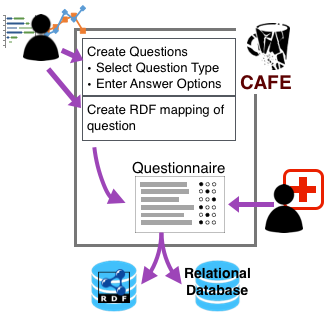
\includegraphics[width=0.28\textwidth]{pics/cafe_process5.png}
  \end{center}
  \caption{CAFE Questionnaire.}
  \label{cafe_process}
\end{wrapfigure}

The result of this work is is available on Github (https://github.com/cafe-trauma/). 
a tool that allows us to create questionnaires, which when they get filled in by the representatives of trauma systems or trauma centers create RDF representations based on the meaning of the answer. 
For example, if the question "Does your trauma center have a trauma registrar?" is answered affirmatively, RDF statements are created to represent the individual trauma registrar role, the bearer of that role (the individual trauma registrar), the individual trauma center in question, and the connections between those entities: the trauma registrar is an organizational member of that trauma center.
To achieve that the questionnaire architect only needs to create the questions, pick the question type (boolean, multi-selection items, drop down menus and entering date or measurement data) .
This application's administrative interface supports creating mappings from questions to RDF templates while constructing the questions for the questionnaire. 
The RDF representations of questions can range from a single RDF statement to a complex set of triples.
In addition to creating RDF triples the answers will  also be recorded in a relational data base.


%TODO JB example would be nice, but space?
When a user answers a question the server-side component will record the answer in the relational database and also insert the configured RDF for that question into the triplestore.
From the user's point of view the questionnaire does not differ in any way from a more typical questionnaire backed by a relational database.
The benefit of this method is that our semantically enriched view of a users organization is available immediately to both build visualizations for the user and to share with public health researchers.
\textcolor{red}{COMMENT, JB: need to say something about what this will be useful for}

\section*{Conclusion}


\makeatletter
\renewcommand{\@biblabel}[1]{\hfill #1.}
\makeatother

\bibliographystyle{unsrt}
\begin{thebibliography}{1}
\setlength\itemsep{-0.1em}

\bibitem{ref1}
T.L.Sanddal,T.J.Esposito,J.R.Whitney,D.Hartford,P.P.Taillac, N. C. Mann NC, et al.. "Analysis of preventable trauma deaths and opportunities for trauma care improvement in Utah," J Trauma. 2011 Apr;70(4):970-7.

\bibitem{ref2}
T. J. Esposito, T. L. Sanddal, S. A. Reynolds, N. D. Sanddal, "Effect of a voluntary trauma system on preventable death and inappropriate care in a rural state," J Trauma, 2003, 54(4), 663-670.

\bibitem{ref3}
Utecht J, Judkins J, Colvin T Jr., et al. OOSTT: a Resource for Analyzing the Organizational Structures of Trauma Centers and Trauma Systems. CEUR Workshop Proc. 2016 Aug;1747. \url{http://ceur-ws.org/Vol-1747/IT504_ICBO2016.pdf}
% is the volume number correct in this citation?



\end{thebibliography}

\end{document}
